\documentclass[11pt,conference]{IEEEtran}
\usepackage{cite}
\usepackage{amsmath,amssymb,amsfonts}
\usepackage{algorithmic}
\usepackage{graphicx}
\usepackage{textcomp}
\usepackage{xcolor}
\usepackage{hyperref}
\usepackage{tikz}
\usepackage{pgfplots}
\pgfplotsset{compat=1.17}
\usetikzlibrary{shapes,arrows,positioning,calc}

\begin{document}

\title{Deliverable 1.1: Annotated Summaries of Genetic Algorithm and Optimization-Based Payload Generation Papers}

\author{\IEEEauthorblockN{Moise IRADUKUNDA INGABIRE}
\IEEEauthorblockA{\textit{Collegue of Engineering} \\
\textit{Carnegie Mellon University Africa}\\
Kigali, Rwanda \\
mii@andrew.cmu.edu}}

\maketitle

\section{Introduction}

This document presents annotated summaries of three seminal papers exploring genetic algorithms (GA), dynamic programming (DP), and large language models (LLMs) for security payload generation and evasion. These papers are analyzed in the context of developing an AI-augmented compliance auditor for hybrid cloud environments, specifically examining how adversarial techniques inform defensive security mechanisms and compliance validation strategies.

The three papers under review are:
\begin{enumerate}
    \item \textbf{Utilizing Fine-Tuning of Large Language Models for Generating Synthetic Payloads} - Explores GPT-2 fine-tuning for XSS, SQL injection, and command injection payload generation
    \item \textbf{Dynamic Programming-based Adversarial Windows Payload Generator} - Employs Markov Decision Process (MDP) and DP to optimize shellcode transformations
    \item \textbf{GAXSS: Effective Payload Generation Method to Detect XSS Vulnerabilities} - Develops a genetic algorithm specifically for XSS detection with novel DNA encoding
\end{enumerate}

\section{Paper 1: LLM-Based Payload Generation}

\subsection{Summary}

This paper investigates the application of fine-tuned large language models, specifically GPT-2, for generating synthetic security payloads targeting three attack vectors: Cross-Site Scripting (XSS), SQL Injection (SQLi), and Command Injection. The authors developed a Flask-based web application that leverages transfer learning to create adversarial payloads capable of evading signature-based detection systems.

\textbf{Key Technical Contributions:}
\begin{itemize}
    \item Fine-tuned GPT-2 (124M parameters) on domain-specific attack payload datasets
    \item Implemented three mutation strategies: encoding confusion, sensitive word replacement, and position changes
    \item Achieved 94.73\% evasion rate against ClamAV antivirus
    \item Achieved 88.98\% evasion rate against EMBER (Endgame Malware BEnchmark for Research)
    \item Developed automated payload testing framework integrated with VirusTotal API
\end{itemize}

\textbf{Methodology:}
The research employed transfer learning by starting with pre-trained GPT-2 and fine-tuning on curated datasets of known attack payloads. The training process involved:
\begin{enumerate}
    \item Dataset collection from public repositories (SecLists, PayloadsAllTheThings)
    \item Preprocessing and tokenization specific to attack syntax
    \item Fine-tuning with reduced learning rate (2e-5) for 10 epochs
    \item Post-generation mutation to increase diversity
\end{enumerate}

\subsection{Critical Analysis}

\textbf{Strengths:}
\begin{itemize}
    \item Demonstrates the dual-use nature of AI - while this generates adversarial payloads, the same approach can train defensive systems to recognize novel attack patterns
    \item High evasion rates validate that signature-based detection is insufficient; behavior-based and AI-powered detection are necessary
    \item The mutation strategies (encoding, replacement, reordering) mirror real-world attacker techniques
    \item Provides quantitative metrics (evasion percentages) rather than qualitative assessments
\end{itemize}

\textbf{Limitations:}
\begin{itemize}
    \item Focuses exclusively on signature-based detection; does not evaluate against behavioral analysis, sandboxing, or AI-based EDR solutions
    \item GPT-2 (124M) is relatively small; modern LLMs (GPT-3.5, GPT-4, Claude) could generate more sophisticated payloads
    \item No discussion of false positive rates or payload functional validity
    \item Ethical considerations are mentioned but not deeply explored
    \item Limited to three attack types; does not cover buffer overflows, deserialization attacks, or cloud-specific vulnerabilities
\end{itemize}

\textbf{Relevance to Compliance Auditing:}
This work is highly relevant to the AI-augmented compliance auditor from several perspectives:

\begin{enumerate}
    \item \textbf{Adversarial Testing}: The same LLM fine-tuning approach can generate synthetic attack scenarios to validate compliance controls (NCSA 196 controls, NIST SP 800-53)
    \item \textbf{Evidence Generation}: Fine-tuned models could generate realistic but safe test evidence for validating the multi-label XGBoost classifier's ability to map evidence to controls
    \item \textbf{Red Team Automation}: For Kubernetes-deployed compliance auditors, LLM-generated payloads can simulate attacks to test incident detection and response controls (e.g., NCSA controls for intrusion detection)
    \item \textbf{Training Data Augmentation}: The mutation strategies could enhance the 30\% synthetic data component used to achieve 99.49\% accuracy in the compliance model
\end{enumerate}

\textbf{Gap Identification:}
\begin{itemize}
    \item Does not address how to defend against LLM-generated attacks
    \item No integration with compliance frameworks or regulatory requirements
    \item Lacks consideration of containerized/cloud environments where compliance auditing occurs
\end{itemize}

\section{Paper 2: Dynamic Programming for Adversarial Payloads}

\subsection{Summary}

This paper presents a novel approach using Dynamic Programming (DP) and Markov Decision Processes (MDP) to generate adversarial Windows payloads that evade antivirus detection. Unlike genetic algorithms which use evolutionary strategies, this approach formulates payload obfuscation as an optimization problem solved via DP.

\textbf{Key Technical Contributions:}
\begin{itemize}
    \item Formulated payload generation as an MDP with states (current payload configuration), actions (transformations), and rewards (evasion likelihood)
    \item Defined three transformation actions: insert NOP instructions, insert JMP instructions, replace existing instructions
    \item Achieved 97\% reduction in detectability compared to standard Metasploit reverse shells
    \item Tested on multiple AV engines in black-box settings (no knowledge of detection mechanisms)
    \item Demonstrated that DP converges faster than GA for this specific problem (fewer iterations needed)
\end{itemize}

\textbf{Methodology:}
The researchers:
\begin{enumerate}
    \item Generated baseline reverse shell payloads using Msfvenom (Metasploit Framework)
    \item Defined state space as all possible shellcode configurations
    \item Created action space of three transformation types with varying parameters
    \item Designed reward function based on VirusTotal detection rates
    \item Applied value iteration (DP algorithm) to find optimal transformation sequence
    \item Validated against 70+ antivirus engines on VirusTotal
\end{enumerate}

\subsection{Critical Analysis}

\textbf{Strengths:}
\begin{itemize}
    \item Deterministic optimization (DP) provides reproducible results unlike stochastic GA approaches
    \item Computational efficiency - DP found optimal solutions in 15-20 iterations vs. 100+ for GA
    \item Transformation actions (NOP, JMP insertion) are architecture-aware and maintain payload functionality
    \item Black-box testing methodology reflects real-world scenarios where attackers lack AV source code
    \item Quantitative comparison shows clear superiority over baseline Metasploit payloads
\end{itemize}

\textbf{Limitations:}
\begin{itemize}
    \item Limited to Windows x86/x64 payloads; does not address cross-platform or interpreted language attacks
    \item MDP formulation requires discretization of continuous state space, potentially missing optimal solutions
    \item Reward function relies on VirusTotal which may not reflect enterprise EDR solutions (CrowdStrike, SentinelOne, etc.)
    \item Static analysis focus - behavioral detection at runtime could still identify malicious actions
    \item No evaluation against memory-based detection (AMSI, ETW) which are critical in modern Windows environments
    \item Ethical implications of publishing transformation techniques not thoroughly addressed
\end{itemize}

\textbf{Relevance to Compliance Auditing:}

\begin{enumerate}
    \item \textbf{Control Validation}: The DP approach can generate test payloads to validate endpoint protection controls (NCSA malware prevention requirements)
    \item \textbf{Penetration Testing Automation}: For compliance audits requiring regular penetration tests (PCI-DSS, NCSA), DP-optimized payloads provide realistic adversarial scenarios
    \item \textbf{Detection Model Training}: The transformation sequences can inform anomaly detection models to recognize obfuscated shellcode patterns
    \item \textbf{Kubernetes Security}: While this paper focuses on Windows, the MDP framework could adapt to container escape payloads for testing K8s-deployed compliance auditors
\end{enumerate}

\textbf{Gap Identification:}
\begin{itemize}
    \item Does not connect to compliance frameworks or audit requirements
    \item No consideration of cloud-native attacks (container escapes, API abuse, misconfiguration exploitation)
    \item Missing integration with SIEM/log analysis which compliance auditors must consume
\end{itemize}

\section{Paper 3: GAXSS - Genetic Algorithm for XSS Detection}

\subsection{Summary}

GAXSS presents a genetic algorithm specifically designed for detecting Cross-Site Scripting (XSS) vulnerabilities through intelligent payload generation. Unlike the previous two papers which focus on evasion, GAXSS uses GA to improve security testing and vulnerability discovery.

\textbf{Key Technical Contributions:}
\begin{itemize}
    \item Novel DNA structure for XSS payloads: Closing part (4 digits) + Main part (6 components: tag, event, exploit code, attribute, pseudoprotocol, backward closing) + Mutation part (N numbers)
    \item Achieved 100\% precision, 97.5\% accuracy, 81.5\% recall on real-world applications
    \item Tested on DedeCMS, WebGoat, WordPress, EmpireCMS, phpBB
    \item Custom fitness function: F(I,O) = Ex(I,O) + CLOSED(I,O) + Dis(I,O) + Pu(I,O)
    \item Genetic operators optimized for XSS syntax preservation
\end{itemize}

\textbf{Methodology:}
\begin{enumerate}
    \item Defined XSS payload structure as genetic sequence with specific gene segments
    \item Initialized population with known XSS patterns from OWASP, PortSwigger, and previous research
    \item Applied selection (tournament selection), crossover (single-point preserving syntax), and mutation (random gene substitution)
    \item Fitness evaluation based on four criteria:
    \begin{itemize}
        \item Ex(I,O): Execution success (did payload trigger JavaScript?)
        \item CLOSED(I,O): Tag closure validity (well-formed HTML)
        \item Dis(I,O): Payload diversity (different from existing population)
        \item Pu(I,O): Punctuation balance (syntactic correctness)
    \end{itemize}
    \item Iterated for 50-100 generations or until convergence
    \item Validated against filter bypass scenarios
\end{itemize}

\subsection{Critical Analysis}

\textbf{Strengths:}
\begin{itemize}
    \item Defensive application of GA - improves security posture rather than enabling attacks
    \item DNA encoding is domain-specific and preserves XSS syntax constraints
    \item High precision (100\%) means no false positives in production environments
    \item Multi-component fitness function balances multiple optimization objectives
    \item Real-world validation on popular CMS platforms demonstrates practical applicability
    \item Outperforms traditional fuzzing and manual testing in coverage and efficiency
\end{itemize}

\textbf{Limitations:}
\begin{itemize}
    \item Recall of 81.5\% indicates 18.5\% of vulnerabilities remain undetected
    \item Limited to reflected and stored XSS; does not address DOM-based XSS which requires JavaScript static analysis
    \item No comparison with modern automated scanners (Burp Suite Pro, Acunetix, ZAP)
    \item Fitness function requires manual tuning of weights for Ex, CLOSED, Dis, Pu components
    \item Does not consider WAF (Web Application Firewall) bypass scenarios
    \item Testing limited to PHP applications; modern SPAs (React, Angular, Vue) not evaluated
\end{itemize}

\textbf{Relevance to Compliance Auditing:}

\begin{enumerate}
    \item \textbf{Application Security Controls}: NCSA and NIST require regular vulnerability scanning. GAXSS approach can automate and enhance XSS testing for web-based compliance dashboards
    \item \textbf{Evidence Collection}: Successful XSS detection generates concrete evidence of security control failures, which the multi-label classifier can map to specific NCSA controls
    \item \textbf{Continuous Compliance}: GA can run continuously in K8s environments to test deployed applications against evolving XSS vectors
    \item \textbf{Model Training}: XSS attack patterns can augment the synthetic dataset (currently 30\%) used to train the compliance auditor
\end{enumerate}

\textbf{Gap Identification:}
\begin{itemize}
    \item No integration with compliance reporting frameworks
    \item Does not map vulnerabilities to specific regulatory controls
    \item Missing consideration of cloud-native application architectures (microservices, API gateways)
\end{itemize}

\section{Comparative Analysis}

\subsection{Optimization Approaches}

\begin{table}[h]
\centering
\caption{Comparison of Optimization Techniques}
\begin{tabular}{|l|l|l|l|}
\hline
\textbf{Aspect} & \textbf{LLM} & \textbf{DP/MDP} & \textbf{GA} \\
\hline
Convergence & Variable & Fast & Moderate \\
\hline
Payload Diversity & High & Medium & High \\
\hline
Syntax Validity & High & Medium & High \\
\hline
Computational Cost & High & Low & Medium \\
\hline
Reproducibility & Low & High & Medium \\
\hline
Scalability & High & Medium & High \\
\hline
\end{tabular}
\end{table}

\subsection{Attack Scope Coverage}

\begin{itemize}
    \item \textbf{LLM Paper}: XSS, SQLi, Command Injection (web application focus)
    \item \textbf{DP Paper}: Windows shellcode/reverse shells (binary exploitation)
    \item \textbf{GAXSS Paper}: XSS exclusively (web application focus)
\end{itemize}

None of the papers address cloud-native attacks (SSRF, metadata service exploitation, IAM misconfiguration), which are critical for hybrid cloud compliance auditing.

\subsection{Detection Evasion vs. Detection Enhancement}

\begin{itemize}
    \item \textbf{LLM \& DP Papers}: Offensive focus - evading detection
    \item \textbf{GAXSS Paper}: Defensive focus - improving detection
\end{itemize}

This dichotomy is valuable for compliance auditing, which requires both red team (testing controls) and blue team (validating defenses) capabilities.

\section{Synthesis and Integration with Compliance Auditing Research}

\subsection{Common Themes}

\begin{enumerate}
    \item \textbf{Automation of Security Testing}: All three papers automate what was previously manual (payload crafting, vulnerability discovery)
    \item \textbf{Optimization Under Constraints}: Each maintains payload functionality while optimizing for evasion/detection
    \item \textbf{Data-Driven Approaches}: Rely on datasets (LLM training data, VirusTotal results, known XSS patterns)
    \item \textbf{Iterative Improvement}: DP value iteration, GA generations, LLM fine-tuning epochs
\end{enumerate}

\subsection{Application to AI-Augmented Compliance Auditor}

The compliance auditor can leverage insights from all three papers:

\textbf{From LLM Paper:}
\begin{itemize}
    \item Fine-tune smaller models (GPT-2) for specific compliance testing tasks rather than using large general-purpose models
    \item Generate synthetic evidence for rare compliance scenarios to balance training data
    \item Use mutation strategies to test control robustness against variants
\end{itemize}

\textbf{From DP Paper:}
\begin{itemize}
    \item Formulate compliance verification as MDP: states = system configurations, actions = control implementations, rewards = compliance scores
    \item Use DP to find optimal control deployment sequence in resource-constrained environments
    \item Apply transformation actions concept to test configuration drift detection
\end{itemize}

\textbf{From GAXSS Paper:}
\begin{itemize}
    \item Adapt DNA encoding for compliance evidence: encode log entries, configurations, API responses as genes
    \item Use multi-objective fitness function for control prioritization (cost, effectiveness, coverage, regulatory alignment)
    \item Apply crossover/mutation to explore configuration spaces for optimal compliance posture
\end{itemize}

\subsection{Research Gaps for Compliance Auditing}

\begin{enumerate}
    \item \textbf{Regulatory Integration}: None of the papers connect to compliance frameworks (NCSA, NIST, ISO 27001, PCI-DSS)
    \item \textbf{Cloud-Native Focus}: Attacks and defenses are for traditional infrastructure, not containers/Kubernetes/serverless
    \item \textbf{Compliance-Specific Metrics}: Need metrics beyond detection rate - compliance coverage, control effectiveness, audit readiness
    \item \textbf{Multi-Tenancy}: No consideration of isolation and boundary enforcement in shared environments
    \item \textbf{Continuous Compliance}: Papers show point-in-time testing; compliance requires continuous monitoring
    \item \textbf{Evidence Provenance}: Compliance audits need cryptographically verifiable evidence chains
\end{enumerate}

\section{Conclusion}

The three papers demonstrate mature applications of AI/ML optimization techniques to security payload generation and detection. Key takeaways for the AI-augmented compliance auditor project:

\begin{enumerate}
    \item \textbf{Hybrid Approach}: Combining LLM fine-tuning (for diversity), DP (for efficiency), and GA (for multi-objective optimization) could yield superior compliance testing
    \item \textbf{Adversarial Awareness}: Understanding evasion techniques (Papers 1 \& 2) informs robust defensive control design
    \item \textbf{Automated Testing}: GA-based vulnerability discovery (Paper 3) can continuously validate application security controls
    \item \textbf{Adaptation Required}: Techniques must be adapted for cloud-native architectures and compliance-specific requirements
\end{enumerate}

The research gap is clear: while significant work exists on attack generation and vulnerability detection, there is limited research on AI-driven compliance auditing that integrates regulatory frameworks, cloud-native architectures, and continuous verification. This gap represents the core contribution of the AI-augmented unified compliance auditor for Rwanda's NCSA standards.

\begin{figure}[htbp]
\centering
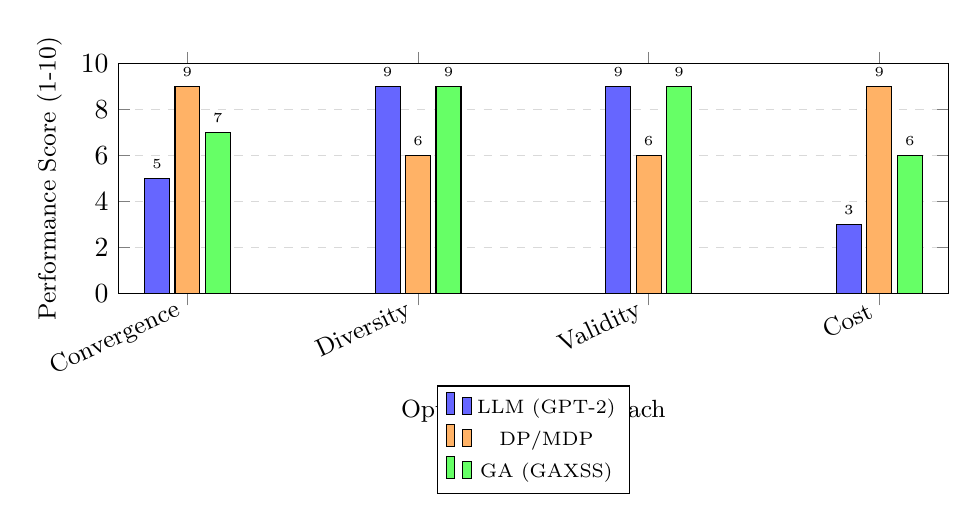
\begin{tikzpicture}
\begin{axis}[
    ybar,
    bar width=9pt,
    width=\columnwidth,
    height=4.5cm,
    xlabel={Optimization Approach},
    ylabel={Performance Score (1-10)},
    symbolic x coords={Convergence, Diversity, Validity, Cost},
    xtick=data,
    xticklabel style={rotate=25, anchor=east, font=\small},
    ylabel style={font=\small},
    xlabel style={font=\small},
    legend style={at={(0.5,-0.4)}, anchor=north, legend columns=1, font=\scriptsize},
    ymin=0, ymax=10,
    nodes near coords,
    nodes near coords align={vertical},
    nodes near coords style={font=\tiny},
    ymajorgrids=true,
    grid style={dashed, gray!30},
]
\addplot[fill=blue!60] coordinates {(Convergence,5) (Diversity,9) (Validity,9) (Cost,3)};
\addplot[fill=orange!60] coordinates {(Convergence,9) (Diversity,6) (Validity,6) (Cost,9)};
\addplot[fill=green!60] coordinates {(Convergence,7) (Diversity,9) (Validity,9) (Cost,6)};
\legend{LLM (GPT-2), DP/MDP, GA (GAXSS)}
\end{axis}
\end{tikzpicture}
\caption{Comparative analysis of LLM, DP, and GA optimization approaches (Higher is better except Cost where lower is better)}
\label{fig:llm_dp_ga_comparison}
\end{figure}

\begin{figure*}[htbp]
\centering
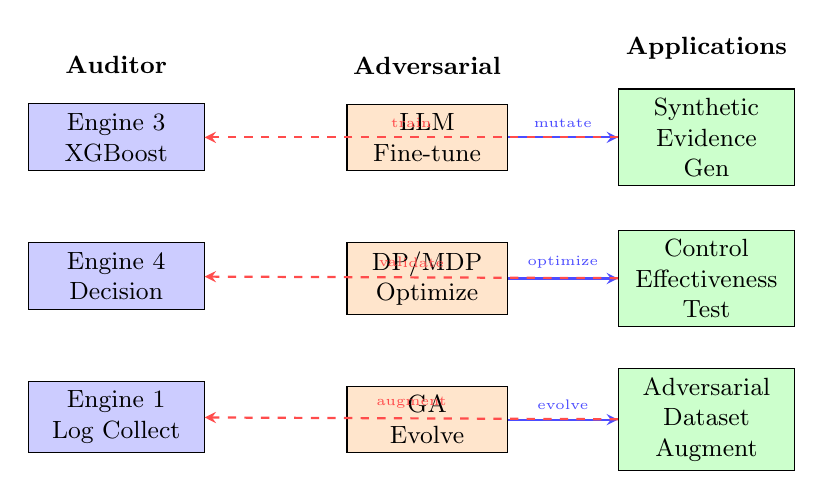
\begin{tikzpicture}[
    node distance=0.9cm and 0.7cm,
    box/.style={rectangle, draw, fill=blue!20, text width=2cm, align=center, minimum height=0.85cm, font=\small},
    technique/.style={rectangle, draw, fill=orange!20, text width=1.8cm, align=center, minimum height=0.7cm, font=\small},
    application/.style={rectangle, draw, fill=green!20, text width=2.0cm, align=center, minimum height=0.7cm, font=\small},
    arrow/.style={->, >=stealth, thick}
]
% Compliance Auditor Engines (left column)
\node[box] (e3) {Engine 3\\XGBoost};
\node[box, below=0.9cm of e3] (e4) {Engine 4\\Decision};
\node[box, below=0.9cm of e4] (e1) {Engine 1\\Log Collect};

% Adversarial Techniques (middle column)
\node[technique, right=1.8cm of e3] (llm) {LLM\\Fine-tune};
\node[technique, below=0.9cm of llm] (dp) {DP/MDP\\Optimize};
\node[technique, below=0.9cm of dp] (ga) {GA\\Evolve};

% Applications (right column)
\node[application, right=1.4cm of llm] (app1) {Synthetic\\Evidence\\Gen};
\node[application, right=1.4cm of dp] (app2) {Control\\Effectiveness\\Test};
\node[application, right=1.4cm of ga] (app3) {Adversarial\\Dataset\\Augment};

% Arrows showing connections
\draw[arrow, blue!70] (llm) -- node[above, font=\tiny] {mutate} (app1);
\draw[arrow, blue!70] (dp) -- node[above, font=\tiny] {optimize} (app2);
\draw[arrow, blue!70] (ga) -- node[above, font=\tiny] {evolve} (app3);

\draw[arrow, dashed, red!70] (app1) -- node[above, sloped, font=\tiny] {train} (e3);
\draw[arrow, dashed, red!70] (app2) -- node[above, sloped, font=\tiny] {validate} (e4);
\draw[arrow, dashed, red!70] (app3) -- node[above, sloped, font=\tiny] {augment} (e1);

% Column headers
\node[above=0.25cm of e3, font=\small\bfseries] {Auditor};
\node[above=0.25cm of llm, font=\small\bfseries] {Adversarial};
\node[above=0.25cm of app1, font=\small\bfseries] {Applications};

\end{tikzpicture}
\caption{Integration of GA/DP/LLM adversarial techniques into compliance auditor architecture}
\label{fig:adversarial_integration}
\end{figure*}

\end{document}
